\chapter{Sanskrit Sandhi}\label{chap:sktsandhi}

Unlike Pāli Sandhi, which is always optional and can be easily learned by acquaintance, Sanskrit Sandhi is inevitable and more complicated. Without the knowledge of Sandhi (euphonic combination), you cannot read Sanskrit texts. The hard part is Sandhi rules are numerous and meticulous. Having tools that can help you understand Sandhi processes is really useful.\footnote{The main source of Sandhi rules used here is Roderick S.\ Bucknell's \emph{Sanskrit Manual} (2004, Motilal Banarsidass). Sandhi grids illustrated in the Manual is really helpful. Another book that uses Sandhi grids (possibly as Bucknell's prototype) is Michael Coulson's \emph{Teach Yourself Sanskrit} (2003, Hodder \& Stoughton).}

Tools related to Sanskrit Sandhi in the program are Sandhi Rules, Sandhi Combiner, and Sandhi Analyzer. The first one is an adaptation of Sandhi grids in tabular form. It is more exhaustive than what can be presented in the grids. The second one has no window of its own. It is an internal function that can be used elsewhere in the program, particularly in Text Editor. The last one can anlyze a string to find Sandhi points.

\section{Sandhi Rules}

This tool, opened by menu Sanskrit > {\faSix \symbol{"F2B5}} Sandhi Rules, is used for looking up how two words are joined together. But what really concerns us is only the ending character of the first word and the beginning of the second. So, you can see a rule of Sandhi like, for example, \pali{-at + i- = -ad i-}.

Here, \pali{t} is the ending of the first word\footnote{Not all consonants are allowed to be final. They are just \pali{k, ṭ, t, p, ṅ, n,} and \pali{m}. All vowels are allowed, also visarga (ḥ), but not anusvāra (ṃ).} (preceded by \pali{a}), plus (+) means `combines with', \pali{i} is the beginning of the second word, equal (=) means `results in', and \pali{-ad i-} is the end product. This can be put simply as ``When \pali{t}, preceded by \pali{a}, meets \pali{i}, it becomes \pali{d}.''

\boxnote{It is a common practice for clarity that even in a combined unit we break the junction in Roman script, like we see in \pali{-ad i-} (not \pali{-adi-}). However, in Devanāgarī the unit is always unbroken (see Figure \ref{fig:sanskrit-sandhi-adi}).
}

\begin{figure}[!hbt]
\centering
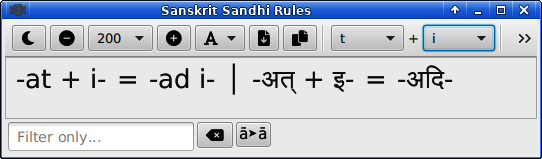
\includegraphics[width=0.8\linewidth]{images/sanskrit-sandhi-adi.png}\\
\caption{Sandhi rule of \pali{-at + i-}}
\label{fig:sanskrit-sandhi-adi}
\end{figure}

Now that you know the basic idea, then we will look at the tool. In the first open, the tool starts with \pali{k} as the ending of the first word, and the beginning of the second word is set to ALL. So, you will see a long table having \pali{k} in the front part. For the preceding vowel has certain effect upon the combination, we have the following options: (1) Only \pali{a}, (2) Only \pali{a \& ā}, and (3) All vowels.

In one case, some ending characters will be doubled if preceded by a short vowel and followed by a vowel (see the results of \pali{-n} and \pali{-ṅ}). That is to say, only \pali{a} and \pali{ā} are enough to see the differences. Adding all vowels can be unnecessarily overwhelming, but you can see the results in all possibilities. In another case, different vowels before ending visarga (ḥ) produce different results (explore the table by yourselves).

The rendition of Devanāgarī is not turned on by default. You have to set it by the option menu button ({\faSix \symbol{"F560}}). Figure \ref{fig:sanskrit-sandhi-rules} shows results from \pali{n} + ALL with \pali{a} and \pali{ā} as preceding vowel, Devanāgarī included.

\begin{figure}[!hbt]
\centering
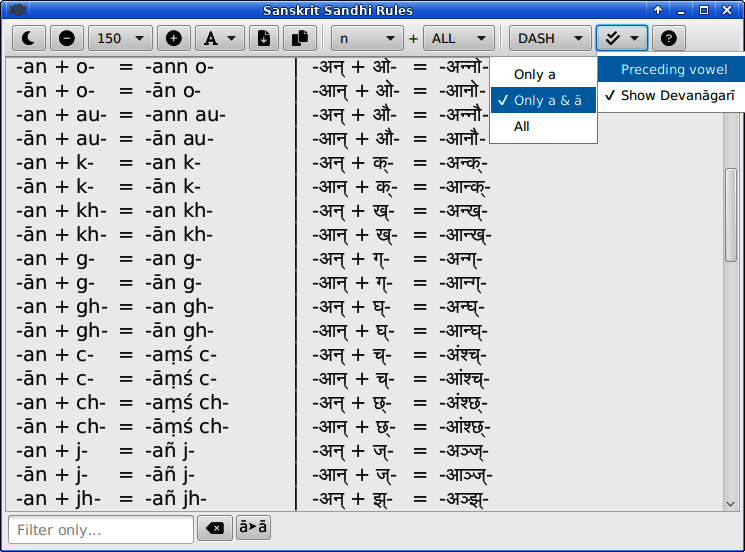
\includegraphics[width=0.9\linewidth]{images/sanskrit-sandhi-rules.png}\\
\caption{Sandhi rules in case of \pali{n} ending}
\label{fig:sanskrit-sandhi-rules}
\end{figure}

If you do not like dashes in the rules, you can eliminate them by setting the output form to BARE. Another option is you can set the output form to WORD. This can make the results look more familiar, but do not take the `word' seriously. It is just a dummy replacement with no meaning whatsoever. Figure \ref{fig:sanskrit-sandhi-wordform} can illustrate the point.

\begin{figure}[!hbt]
\centering
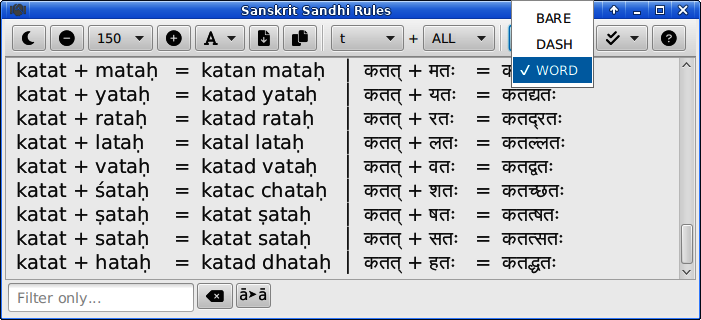
\includegraphics[width=0.9\linewidth]{images/sanskrit-sandhi-wordform.png}\\
\caption{Using word-formed output in Sandhi table}
\label{fig:sanskrit-sandhi-wordform}
\end{figure}

Another feature is very helpful when you want to see a specific combination or product. You can use finding tool at the bottom. A typical use case is when you select both the ending and beginning character to ALL and search for a pattern. Figure \ref{fig:sanskrit-sandhi-find} shows findings: (a) in combinations (a plus sign is used), and (b) in products (a space is used).

\begin{figure}[!hbt]
\centering
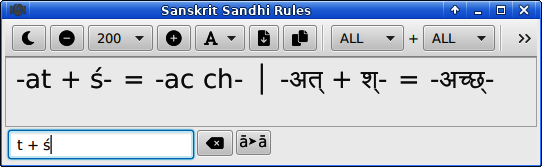
\includegraphics[width=0.8\linewidth]{images/sanskrit-sandhi-find1.png}\\
(a) Finding in combinations\\[3mm]
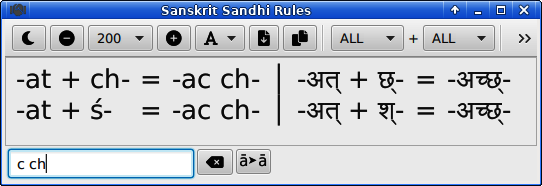
\includegraphics[width=0.8\linewidth]{images/sanskrit-sandhi-find2.png}\\
(b) Finding in products\\
\caption{Finding in Sandhi table}
\label{fig:sanskrit-sandhi-find}
\end{figure}

\section{Sandhi Combiner}

In a real world application of Sandhi, you have two words and you want to make them combined. Manually, you have to know the rule concerning the ending and beginning of the words, then you apply the rule accordingly. Now we have the tool for looking up Sandhi rules mentioned above, otherwise you have to look up at Sandhi grids.

The main benefit of having a computer is we can make it compute the results for us. That is what Sandhi Combiner does in the program. The combiner is not a specific tool. It is just a function that can be used in the program. To use this to combine two words, you have to do it in Text Editor. Figure \ref{fig:sanskrit-sandhi-combine} shows \pali{āsīt śatruḥ} (There was an enemy) in an Editor. You can make two words combined with menu Tools > Sandhi > Sanskrit combine. The product of this is shown in Figure \ref{fig:sanskrit-sandhi-product}.

There are conditions the users should know as follows:

\begin{compactenum}
\item Devanāgarī conversion is automatically done and placed in a line below.
\item If more than two words are present, all the words are combined at once.
\item If there are alternatives in the combination, all products are shown.
\item The computation is done line by line. So, you can process several combinations at once by entering them in different lines.
\end{compactenum}

\begin{figure}[!hbt]
\centering
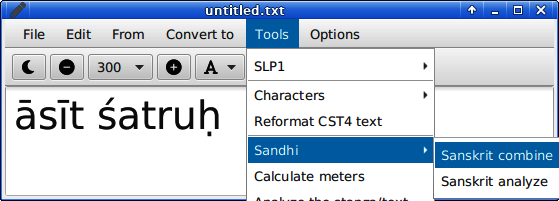
\includegraphics[width=0.8\linewidth]{images/sanskrit-sandhi-combine.png}\\
\caption{Combining two words in Text Editor}
\label{fig:sanskrit-sandhi-combine}
\end{figure}

\begin{figure}[!hbt]
\centering
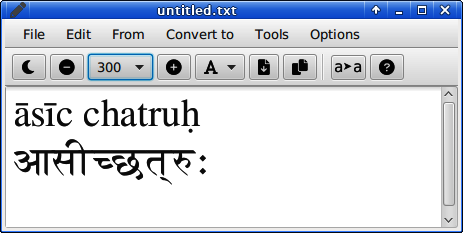
\includegraphics[width=0.8\linewidth]{images/sanskrit-sandhi-product.png}\\
\caption{Product of a Sandhi combination}
\label{fig:sanskrit-sandhi-product}
\end{figure}

\section{Sandhi Analyzer}

A combination of two words into one Sandhi unit according to the rules is straightforward and simple, but the reverse is more complicated because there are possibilities that on product of Sandhi may come from several combinations. So, analyzing Sandhi is difficult by its nature, particularly with a long unit.

To do an analysis, you can simply select a Sandhi unit (either Roman or Devanāgarī) in Text Editor and use menu Tools > Sandhi > Sanskrit analyze (see Figure \ref{fig:sanskrit-sandhi-analyze}). In the picture, it is the product of Sandhi combination we have done in the previous section. 

\begin{figure}[!hbt]
\centering
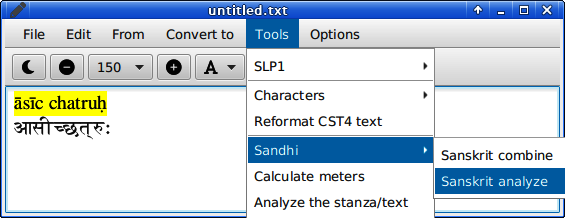
\includegraphics[width=0.8\linewidth]{images/sanskrit-sandhi-analyze.png}\\
\caption{Starting Sandhi analysis from Text Editor}
\label{fig:sanskrit-sandhi-analyze}
\end{figure}

Another way to start an analysis is you have to copy the string to the system's clipboard first. Figure \ref{fig:sanskrit-sandhi-copy} shows the context menu in the program's Text Editor. You can do likewise in other editors or applications (usually with \texttt{Ctrl-C}). Then you open the Analyzer by menu Sanskrit > {\faSix \symbol{"F6E3}} Sandhi Analyzer, and press {\faSix \symbol{"F0EA}} button, either in the top tool bar or the small tool bar. As a result, you should see things as shown in Figure \ref{fig:sanskrit-sandhi-analyzer-result}.

\begin{figure}[!hbt]
\centering
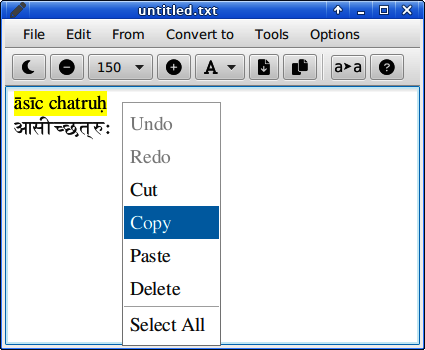
\includegraphics[width=0.6\linewidth]{images/sanskrit-sandhi-copy.png}\\
\caption{Copying a Sandhi unit from Text Editor}
\label{fig:sanskrit-sandhi-copy}
\end{figure}

\begin{figure}[!hbt]
\centering
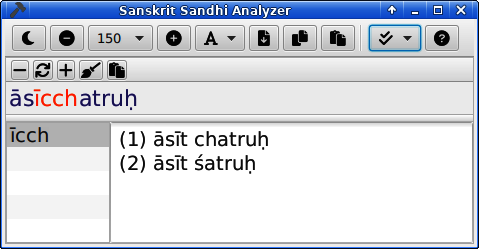
\includegraphics[width=0.8\linewidth]{images/sanskrit-sandhi-analyzer-result.png}\\
\caption{Sandhi Analyzer showing a result}
\label{fig:sanskrit-sandhi-analyzer-result}
\end{figure}

The process of analysis can be described as follows:

\begin{compactenum}
\item The Sandhi unit, even broken in the source, is connected.
\item Analyzable junctions are listed on the left pane. The selected one is highlighted.
\item The result is shown on the right pane. If multiple combinations are found, they are listed with numbers.
\item You can clear the analysis with {\faSix \symbol{"F51A}} button. Or you can start a new analysis right away by copying a new string to the tool.
\end{compactenum}

The result shown above tell us that \pali{āsīc chatruḥ} may come from either \pali{āsīt + śatruḥ} or \pali{āsīt + chatruḥ}. However, because \pali{chatruḥ} has no meaning (luckily), the only possible combination is therefore \pali{āsīt + śatruḥ}. Here is an optimistically simple example, by which the tool can really help. But a real life application is more complicated than that.

Figure \ref{fig:sanskrit-sandhi-analyzer-rules} show results from analyzing \pali{śuklāmbaradharaṃ}. At first you may see less than what I show you. Once you enable more rules in analysis, more results emerge, sometimes overwhelmingly. You have to choose the right result yourselves by using dictionaries.

\newpage
\begin{figure}[!hbt]
\centering
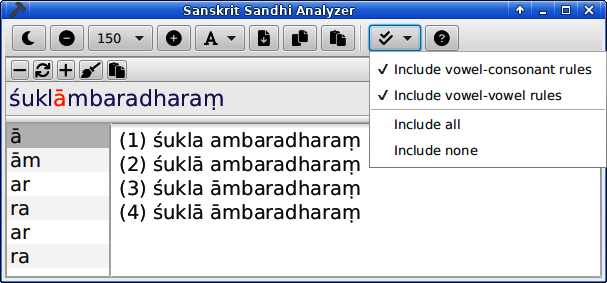
\includegraphics[width=0.9\linewidth]{images/sanskrit-sandhi-analyzer-rules.png}\\
\caption{Including more rules in Sandhi Analyzer}
\label{fig:sanskrit-sandhi-analyzer-rules}
\end{figure}

